%; whizzy chapter
% -initex iniptex -latex platex -format platex -bibtex jbibtex -fmt fmt
% 以上 whizzytex を使用する場合の設定。


%     Tokyo Debian Meeting resources
%     Copyright (C) 2009 Junichi Uekawa

%     This program is free software; you can redistribute it and/or modify
%     it under the terms of the GNU General Public License as published by
%     the Free Software Foundation; either version 2 of the License, or
%     (at your option) any later version.

%     This program is distributed in the hope that it will be useful,
%     but WITHOUT ANY WARRANTY; without even the implied warranty of
%     MERCHANTABILITY or FITNESS FOR A PARTICULAR PURPOSE.  See the
%     GNU General Public License for more details.

%     You should have received a copy of the GNU General Public License
%     along with this program; if not, write to the Free Software
%     Foundation, Inc., 51 Franklin St, Fifth Floor, Boston, MA  02110-1301 USA

%  preview (shell-command (concat "evince " (replace-regexp-in-string "tex$" "pdf"(buffer-file-name)) "&"))
% 画像ファイルを処理するためにはebbを利用してboundingboxを作成。
%(shell-command "cd image200906; ebb *.png")

%%ここからヘッダ開始。

\documentclass[mingoth,a4paper]{jsarticle}
\usepackage{monthlyreport}

% 日付を定義する、毎月変わります。
% date --date 'third saturday'
\newcommand{\debmtgyear}{2009}
\newcommand{\debmtgmonth}{6}
\newcommand{\debmtgdate}{20}
\newcommand{\debmtgnumber}{53}

\begin{document}

\begin{titlepage}
\thispagestyle{empty}

% タイトルページ:編集必要な部分は最初のマクロに飛ばすこと

\vspace*{-2cm}
第\debmtgnumber{}回 東京エリア Debian 勉強会資料

\hspace*{-2.4cm}
\includegraphics[width=210mm]{image200801/2008title.eps}\\
\hfill{}\debmtgyear{}年\debmtgmonth{}月\debmtgdate{}日

\end{titlepage}

\dancersection{Introduction}{上川 純一}

\begin{multicols}{2}
 
 
 今月のDebian勉強会へようこそ。これからDebianの世界にあしを踏み入れると
 いう方も、すでにどっぷりとつかっているという方も、月に一回Debianについ
 て語りませんか?

 Debian勉強会の目的は下記です。

 \begin{itemize}
 \item \underline{Debian Developer} (開発者)の育成。
 \item 日本語での「\underline{開発に関する情報}」を整理してまとめ、アップデートする。
 \item \underline{場}の提供。
 \begin{itemize}
  \item 普段ばらばらな場所にいる人々が face-to-face で出会える場を提供
	する。
  \item Debian のためになることを語る場を提供する。
  \item Debianについて語る場を提供する。
 \end{itemize}
 \end{itemize}		

 Debianの勉強会ということで究極的には参加者全員がDebian Packageをがりがり
 と作るスーパーハッカーになった姿を妄想しています。情報の共有・活用を通し
 て Debianの今後の能動的な展開への土台として、「場」としての空間を提供す
 るのが目的です。

 2009年の計画は仮です。

 \begin{enumerate}
  \item 新年の企画 (アンサンブル荻窪開催)
  \item OSC Tokyo
  \item VAIO P インストール記録、
	カーネル読書会 ディストリビューション大集合(小林さん)(東京大学?)
  \item Git Handson (岩松)(あんさんぶる荻窪?)
  \item 家Debianサーバ vs 職場のネットワーク(千代田区都立図書館?\footnote{\url{http://www.library.chiyoda.tokyo.jp/}})
  \item Asterisk (東京大学?)
  \item スペインにて開催
  \item Debconf報告会
  \item OSC Fall?
  \item udev + HAL(岩松さん)
  \item 3D graphics 開発(藤沢さん) 
  \item Debian サーバ+VMware + 各種OS、
	他の仮想化ツール(vserver etc.)、
	忘年会
 \end{enumerate}

 会場候補としては下記があります:

 \begin{itemize}
  \item 大学
  \item 恵比寿SGIホール
  \item Googleオフィス
  \item 公民館(あんさんぶる荻窪等)
  \item 都立会議室(無線LAN)
  \item 健保の施設
 \end{itemize}

\end{multicols}


\newpage

\begin{minipage}[b]{0.2\hsize}
 \definecolor{titleback}{gray}{0.9}
 \colorbox{titleback}{\rotatebox{90}{\fontsize{80}{80} {\gt デビアン勉強会} }}
\end{minipage}
\begin{minipage}[b]{0.8\hsize}
\hrule
\vspace{2mm}
\hrule

% set depth to 1 if too many text, 2 if there's less
\setcounter{tocdepth}{1}
\tableofcontents
\vspace{2mm}
\hrule
\end{minipage}

\dancersection{事前課題}{上川 純一}

事前課題は:

DDTSS (先月のPDF資料 今月のPDF資料参照)でいくつか(2個以上)Debianパッケージの説明文を翻訳してみて、いくつか(2個以上)レビューしてみて、そこでの

\begin{enumerate}
 \item 作業に適用した主要な方法
 \item 発見した課題
 \item 方法の改善案の提案をしてください。
\end{enumerate}

この課題に対して提出いただいた内容は以下です。

\begin{multicols}{2}
%; whizzy-master ../debianmeetingresume200906.tex
% $B0J>e$N@_Dj$r$7$F$$$k$?$a!"$3$N%U%!%$%k$G(B M-x whizzytex $B$9$k$H!"(Bwhizzytex$B$,MxMQ$G$-$^$9!#(B

\begin{prework}{$B>e@n=c0l(B}
...
\end{prework}



\begin{prework}{$B@nK\7rB@O:(B}
\preworksection{$BE,MQ$7$?<gMW$JJ}K!(B}

2009/06$B$N;qNA$N!V(BDDTSS$B$NK]Lu:n6H$N>R2p!W$r;29M$K!"(B
DDTSS $B$K%f!<%6!<EPO?$7!"?7$7$$K]Lu!&=$@5!&%l%S%e!<$r(B3$B$D$:$D9T$$$^$7$?!#(B


\preworksection{$BH/8+$7$?2]Bj(B}

\begin{itemize}
 \item "Accept with changes" $B$9$k$H!"%l%S%e!<%W%m%;%9$,$d$jD>$7$K$J$k$N$G!"$A$g$C$H$7$?=$@5(B ($B6gFIE@$NDI2C$J$I(B) $B$,$G$-$J$$(B
 \item ($B$=$NA0$N9F$H$N:9J,$@$1$G$O$J$/(B) $B:G?79F$b8+$?$$(B
 \item $BK]Lu$N4p=`$,$o$+$i$J$$$N$G!"(BSubmit$B$7$FNI$$$N$+<+?.$,;}$F$J$$(B
 \item DDTSS$B$N%5!<%P>ZL@=q$,IT@5(B
 \item Alias$B$N%k!<%k$,EPO?;~$H%m%0%$%s;~$H$G0[$J$k(B ($BEPO?;~$O(B "at least 4 letter long" $B$G%m%0%$%s;~$O(B "at least 6 letter long")
\end{itemize}

3 $BE@L\$O?4M}E*$JLdBj$G$9$,!"(B
$B$I$N%l%Y%k$NK]Lu$r5a$a$i$l$F$$$k$N$+$o$+$i$J$$$N$G!"(B
Submit $B$r$?$a$i$C$F$7$^$$$^$7$?!#(B
($B$H$O$$$(!":G=*E*$K$O(B Submit $B$7$^$7$?$,!#(B)
$B8mLu$,$J$$$N$OEvA3$H$7$F$b!"@lLgMQ8l$NLu$d!"(B
$BF|K\8l$H$7$F$N<+A3$5$J$I!"K]Lu$N<A$,5$$K$J$C$F$7$^$$$^$9!#(B

\preworksection{$BDs0F$9$kM}A[A|(B($B%D!<%k$H$+(B)$B!"6&M-$7$?$$>pJs(B}

$B>e5-2]Bj$N(B 1 $BE@L\$NBP:v$H$7$F!"(B
"Change and restart review process" $B$H(B "Accept with minor changes" $B$H$N(B
2 $B$D$,J,$+$l$F$$$l$PNI$$$H;W$$$^$9!#(B
$B!V$o$:$+$J=$@5$G$b!"%l%S%e!<%W%m%;%9$r$d$jD>$9!W$H$$$&$N$O!"(B
$B87L)@-$rJ]$D$?$a$K$OI,MW$G$9$,!"(B
"The number of translations pending review has gotten quite large." $B$H$$$&>u67$G!"(B
$B6gFIE@0l$DD>$9$?$S$K!"$^$?(B 3 $B?M$N%l%S%e!<%o$,I,MW$K$J$k$N$O8=<BE*$G$O$J$$$H;W$$$^$9!#(B
$B5U$K!"%l%S%e!<%o$,$A$g$C$H$7$?=$@5$r$"$-$i$a$k$3$H$G!"(B
$B%I%-%e%a%s%H$,$A$g$C$HFI$_$K$/$/$J$k$N$O;DG0$G$9!#(B


\end{prework}

\begin{prework}{$B$^$($@$3$&$X$$(B}

\preworksection{$BE,MQ$7$?<gMW$JJ}K!(B}

$B$3$3$G$N(B''$BJ}K!(B''$B$,2?$r0U?^$7$F$$$k$N$+$,J,$+$i$J$$$N$G!"%D!<%k$N;H$$J}$G(B
 $B$O$J$/!"K]Lu$N$d$jJ}$H$$$&4QE@$G=q$-$^$9!#K]Lu$N$d$jJ}<+BN$O!"K]LuDL?.(B $BJL:}!X?N(B
 $BJ?OBIW>.O@=8(B $BK]Lu$N%3%D!Y(B
 \footnote{\url{http://homepage3.nifty.com/hon-yaku/tsushin/bn/200209SAp2.pdf}}
 $B$r;29M$K$7$^$7$?!#%3%D$O?'!9$"$k$h$&$G$9$,!"$$$/$D$b0U<1$9$k$N$OFq$7$$(B
 $B$N$G!"<!$N;0E@$@$1$O0U<1$9$k$h$&$K$7$^$7$?!#(B

\begin{itemize}
 \item $BD>Lu$K$O$7$J$$$G!"F|K\8l$H$7$F$o$+$j$d$9$$J8>O$r?4$,$1$k!#(B
 \item $BD9J8$GJ,$+$j$E$i$1$l$P!"C;J8$KJ,3d$7$F$_$k!#(B
 \item $B7AMF;l$,O"H/$5$l$F$$$kItJ,$O0U?^E*$KLu$5$J$$!#(B
\end{itemize}

\preworksection{$BH/8+$7$?2]Bj(B}

 $B$^$:!"%7%9%F%`E*$J$3$H!#(B

 $B%m%0%$%s$7$J$/$F$b(B $B%l%S%e!<!"=$@5$G$-$F$7$^$C$?$N$G!"(BID $B$r:n$C$F$$$?$K(B
 $B$b4X$o$i$:!"(Bcokkie $B$K;D$C$?>pJs$G%"%/%;%9$7$F$$$k$N$+$H;W$$$=$N$^$^(B
 Accept $B$9$k$H!"(BID $B$,(B IP $B%"%I%l%9$K$J$C$F$7$^$&$H$$$&$A$g$C$H%^%L%1$J<+(B
 $BBN$K!#(B


 $B$b$&0l$D$O!"@lLgMQ8l$K$D$$$F!#85!9Bg3X$,@8J*3X2J$G$7$?$N$G!"@8J*4XO"$N(B
 $B@lLgMQ8l$K8BDj$7$FOC$r$7$^$9!#3X@8;~J,$K!"0lHV:$$C$?$N$O1Q8l$NJ8=q$7$+(B
 $B$J$$$3$H$G$O$J$/$F!"JQ$JK]Lu$N$5$l$+$?$r$7$F$$$kMQ8l!"FC$K%+%?%+%J$KK](B
 $BLu$5$l$F$$$kMQ8l$G$9!#(B

 $B@lLgMQ8l$rD4$Y$k$N$K$O!"DL>o!"@lLgMQ8l$N<-=q$r;H$$$^$9!#@8J*$@$H@8J*3X(B
 $BA4HL!"@82=3X!"7OE}J,N`3X!"J,;R@8J*3X!"$J$I$J$I!"3FJ,Ln$G@lLg$N<-=q$,$"(B
 $B$j$^$9$,!"JQ$KK]Lu$5$l$F$$$k$H!":w0z$+$i0z$/$3$H$,$G$-$^$;$s!#$G$9$N$G!"(B
 $B@lLgMQ8l$rD4$Y$k$H$-$O!"86J8!J1Q8l$+!"3XL>$G;H$o$l$k%i%F%s8l!K$GD4$Y$k(B
 $B$N$,4pK\$G$9!#(B

\preworksection{$BDs0F$9$kM}A[A|(B($B%D!<%k$H$+(B)$B!"6&M-$7$?$$>pJs(B}

 $BA0<T$K$D$$$F$O!"(BDDTSS$B$K%m%0%$%s$7$J$$$HJQ99$G$-$J$$$h$&$K%j%/%(%9%H$r=P(B
 $B$9$N$,$h$$$N$G$7$g$&$+!D!#(B


 $B8e<T$K$D$$$F$O!"$"$1$I$5$s$,:#2s$*OC!"Ds8@$7$F$/$@$5$k$H;W$$$^$9$,!"0lHL(B
 $B?M8~$1$KK]Lu$O$9$k$b$N$N!"86J8$O3g8L=q$-$J$I$G8e$m$K;D$7$F$*$/$N$,<B:](B
 $B$K;H$&%f!<%6!J$=$NJ,Ln$N@lLg2H!K$K$O?F@Z$@$H;W$$$^$9!#(B

\end{prework}


\begin{prework}{$B$"$i$-$d$9$R$m(B}

\preworksection{$BE,MQ$7$?<gMW$JJ}K!(B}

$B$H$/$K$J$$$+$J$"!#$R$?$9$iK]Lu!#(B

\preworksection{$BH/8+$7$?2]Bj(B}

$B%Q%C%1!<%8L>$$$-$J$j$8$c$J$/$F!"%Q%C%1!<%8$N=jB0$9$k(Bsection$B$,$+$+$l$F$$$k$H3Z$J(B
$B$N$K$J$"!"$H;W$$$^$7$?!#(B
review$B$,$*$b$$$N$[$+4JC1$H$$$&$+!"$Y$D$K(Bdd$B$,$R$H$j$b4X78$7$J$/$F$b$$$$$s$G$9$M!#(B
$B$"$k0UL#$*$I$m$-$+$b!#(B

\preworksection{$BDs0F$9$kM}A[A|(B($B%D!<%k$H$+(B)$B!"6&M-$7$?$$>pJs(B}

$BD6$`$+$7(B(1997$B$3$m(B)$B$K$3$N<j$N:n6H$r$7$?$H$-$H$O$<$s$<$s0c$$$^$9$M!#(B
$B$G$b!"$"$$$F$k;~4V$K$d$j$?$$$H$-$b$"$k$N$G%*%s%i%$%s$G$O$J$/%P%C%A=hM}$G$-$k;EAH(B
$B$b$N$3$C$F$k$H$&$l$7$$$+$J$H!#(B

\end{prework}


\end{multicols}

% image200906/prework.tex 内部にテキストを追加してください。
%
%

\dancersection{最近のDebian関連のミーティング報告}{上川 純一}
\subsection{東京エリアDebian勉強会52回目報告}
% (query-replace-regexp "<.*?>" "")
% (query-replace-regexp "^[	 ]\+" "")

東京エリアDebian勉強会報告。2009年5月16日土曜日に東京エリアDebian勉強会の
第52回を練馬区のサンライフ練馬にて開催しました。隣の部屋からは三味線と謡
(?)の練習の音が聞こえる和室での開催、和やかな雰囲気でした。今回の参加者は
あけど, 山本, 小室, 日比野, でん, きたはら, 前田, 藤澤徹, やまだたくま,
吉田@板橋, 高橋(masaka), やまねひでき, 上川 x 2 の14名でした。

まず、クイズ。

藤澤徹さんがMCMPIパッケージをITPしてみたので報告。
一歩一歩公式パッケージ化に進んでいるようです。

前田さんが erlang を使ってみたので報告。
Debianでどのパッケージをいれたら動くのかはわかりました。

上川がAndroid開発環境をDebianをつかってみたので報告。とりあえずデモアプリ
を動かすことができました。

その後、DDTSSのワークフローについてディスカッション。過去の経緯から掘り起
こして語って見ました。2003年くらいからすでにDebian Descriptionを翻訳する
ためのフレームワークDDTPは登場していたのですが、利用する側の仕組みが十分
整備されていませんでした。2008年くらいにapt側もDebian アーカイブ側も翻訳
をサポートしたのでそろそろやってみるか、と眺めてみました。10年前に議論し
た結果をまとめたDebian JPの文書作成の指針という文書
(\url{SVN:www/trunk/src/community/translate/debiandoc-guidelines-ja/debiandoc-guidelines-ja.sgml})
があるだとか、当時作成したSKK形式で用語の対訳表
(\url{SVN:www/trunk/src/community/translate/trans_table/table.skk}) があ
るだとかいう話題が出ました。議論するための情報が十分集約されていないので
継続して、来月は資料を準備しなおしてあらためてこのテーマで議論することに
なりました。

宴会は駅前の「のみくい処 仲々」にて。


%============================================================
%%% trivia quiz
\dancersection{Debian Trivia Quiz}{上川 純一}

ところで、みなさん Debian 関連の話題においついていますか?Debian関連の話
題はメーリングリストをよんでいると追跡できます。ただよんでいるだけではは
りあいがないので、理解度のテストをします。特に一人だけでは意味がわからな
いところもあるかも知れません。みんなで一緒に読んでみましょう。

今回の出題範囲は\url{debian-devel-announce@lists.debian.org} に投稿された
内容とDebian Project Newsからです。

\begin{multicols}{2}
 %; whizzy-master ../debianmeetingresume200906.tex
% $B0J>e$N@_Dj$r$7$F$$$k$?$a!"$3$N%U%!%$%k$G(B M-x whizzytex $B$9$k$H!"(Bwhizzytex$B$,MxMQ$G$-$^$9!#(B
%
% $B$A$J$_$K!"%/%$%:$OJL%V%i%s%A$G:n@.$7!"$N$A$K%^!<%8$7$^$9!#5U$K%^!<%8$7(B
% $B$J$$$h$&$K$7$^$7$g$&!#(B
% (shell-command "git checkout quiz-prepare")

\santaku
{$B%h!<%m%C%Q$K?7@_$5$l$?%"%C%W%m!<%I%-%e!<$NL>A0$O(B?}
{ftp.eu.upload.debian.org}
{ftp.uk.upload.debian.org}
{ftp.jp.debian.org}
{A}
{}

\santaku
{$B?7$7$$%"%C%W%m!<%I%-%e!<$G?7$7$/%5%]!<%H$9$k$3$H$K$J$kDL?.%W%m%H%3%k$O(B?}
{ipv6}
{sstp}
{RFC2324} % coffee protocol
{A}
{}

\santaku
{GPG $B%-!<:F:n@.:W$j$O$J$<H/@8$7$?$+(B?}
{$B$=$m$=$m(Bsha-1$B$,@H<e$K$J$C$?$H;W$o$l$k$+$i(B}
{$BOG@1$,D>Ns$9$k$+$i(B}
{GPG$B$,<+M3$G$J$/$J$C$?$+$i(B}
{A}
{}

\santaku
{packages.debian.org $B%a!<%k$K$D$$$F2?$,%"%J%&%s%9$5$l$?$+(B}
{debian.org$B0J30$+$i%a!<%k$r<u?.$7$J$/$9$k(B}
{debian.org$B0J30$+$i$7$+%a!<%k$r<u?.$7$J$/$9$k(B}
{debian.net$B0J30$+$i%a!<%k$r<u?.$7$J$/$9$k(B}
{A}
{}

\santaku
{eeePC$B$O(B5$B7n;~E@$G2?5!<o$"$k$+(B}
{16}
{24}
{32}
{B}
{}

\santaku
{Debian $B$,(B glibc $B$NBe$o$j$K:NMQ$9$k$HH/I=$7$?(B libc $B$O$J$K$+(B}
{newlib}
{eglibc}
{BSD libc}
{B}
{}

\santaku
{debian-cli $B$H$$$&%a!<%j%s%0%j%9%H$O2?$r$9$k$H$3$m$+(B?}
{command line interface $B$K$D$$$F8l$k>l=j(B}
{common language infrastructure $B$K$D$$$F8l$k>l=j(B}
{cat-linux interface $B$K$D$$$FLQA[$9$k>l=j(B}
{B}
{}

\santaku
{Debian policy 3.8.2 $B$G$+$o$C$?E@$O$I$l$+!#(B}
{debconf $BI,?\(B}
{X $B$OGQ;_$K$J$j$^$7$?(B}
{MS EULA $B$,G'Dj%i%$%;%s%9$K4^$^$l$?(B}
{A}
{}

\santaku
{gluck $B$O$$$DGQ;_$K$J$k$+(B}
{6$B7nKv(B}
{Squeeze$B%j%j!<%9;~(B}
{Lenny $B%j%j!<%9;~(B}
{A}
{}

\end{multicols}


% ===============================================================
\dancersection{DDTP 翻訳作業での TIPS}{あけど}
\index{DDTSS}
\index{DDTP}
% ===============================================================

\subsection{はじめに}


Debian Package をインストールする際に参考する情報、``Description'' 昔は
すべて英語でしたが、最近はすこしづつ日本語になってきているのはご存知でし
たか?
Debian Description Translation Project は Debian Package の Description
文(パッケージの内容を説明する文章)を日本語にするためのプロジェクトです。
\footnote{DDTPサイト: \url{http://ddtp.debian.net/}}

日本語の翻訳の進捗は図 \ref{fig:transstatja} の状況です。

\begin{figure}[h]
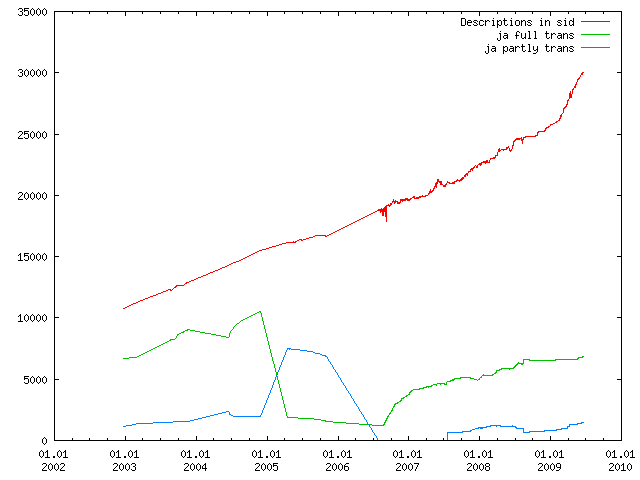
\includegraphics[width=0.5\hsize]{image200906/stat-trans-sid-ja.png}
\caption{日本語の状況}
\label{fig:transstatja}
\end{figure}

前回、5月の東京エリアDebian勉強会でトピックに挙っていました DDTSS につい
て、作業上の留意点などをまとめてみました。DDTSS については運用ルールなど
で明確になっていない部分もありますので、その議論を深める材料になればと思います。
このセクションはこれから翻訳を始めてみようという方へのガイドとしても考慮した
つもりです。
なお、このセクションにおいての幾つかの見解は筆者の個人的見解が多分に含まれて
いますので、その点ご留意頂ければと存じます。

\url{http://tokyodebian.alioth.debian.org/pdf/debianmeetingresume200905.pdf}
 p.31「8 DDTSS 活用」

\subsection{ガイド等の文書の把握}
5月の資料にまとまっていますが、その後に作成されたページをご案内します。

\begin{itemize}
 \item DDTSS\_ja/Faq - Debian Wiki
% ja/DDTSS_ja/Faq - Debian Wiki
       \url{http://wiki.debian.org/ja/DDTSS_ja/Faq}
\end{itemize}

以下は5月の再掲です。
\begin{itemize}
 \item Debian パッケージの説明文を日本語で読みたい! 〜DDTP へのお誘い〜 
       \url{http://www.debian.or.jp/community/translate/description-ja.html}
 \item 武藤健志さんのblogの『Debianドキュメント翻訳手続き』:
       \url{http://kmuto.jp/d/index.cgi/debian/debian-doc-procedure.htm}
 \item 小林儀匡さんのDebian勉強会2006年9月資料「翻訳への誘い」:
       \url{http://tokyodebian.alioth.debian.org/pdf/debianmeetingresume200609.pdf}
 \item debian-doc メーリングリスト:
       主要な議論が行われています。質問なども、こちらで。
\end{itemize}

\subsection{翻訳(辞書)サイトの利用}
翻訳するのに十分な知識があればそもそも辞書は必要無いのかも知れません。
印刷された辞書を使うのはインターネット接続がない環境では有効ですが、
コンピュータを使う現代的な環境であればインターネット接続はほぼ不可欠でしょうから、
オンラインの翻訳サイトを利用しない手はありません。
以下にお勧めのサイトをご紹介します。

\begin{itemize}
 \item{英単語辞書
  \begin{itemize}
   \item{英辞郎 on the web スペースアルク \url{http://www.alc.co.jp/}
収録単語の量、質、訳がそれぞれ秀逸です。
スラング等の現代語から専門用語まで幅広く、また対象の英単語が含まれる例文が実例に基づいていて実用的な訳を得られます。
(※このサイトを利用しているだけで、中学、高校で受けた英語が英文学を主眼に置いたものだと実感しました。)}
  \end{itemize}
 }
 \item{文章翻訳
  \begin{itemize}
   \item{Yahoo!翻訳 \url{http://honyaku.yahoo.co.jp/}
   文単位での訳と原文の対応が付くので、長い文章や複雑な文章の翻訳に向いています。}

   \item{英語翻訳 - エキサイト 翻訳
     \url{http://www.excite.co.jp/world/}
   自然な表現の日本語訳を得られます。カタカナ語の訳語をかなり上手く当てはめてくれたりします。}

   \item{Cross Translation::色々な翻訳サイト・翻訳サービスの一括、横断翻訳
     \url{http://sukimania.ddo.jp/trans/trans.php}
   上記のYahoo!翻訳、エキサイト 翻訳などの翻訳サービスにて一括で翻訳するサービスです。
   翻訳に迷った時の参考になるでしょう。但し、全てのサイトでの結果を得るには多少時間がかかります。}
  \end{itemize}
  他にも辞書・翻訳サイトは多数ありますので、各自で探してみて下さい。
 }
\end{itemize}


\subsection{Google で 「Debian」+「対象のパッケージ名」を検索}
Debian パッケージの過去バージョンで既に翻訳されている事がありますので
それを参考にすることもできます。

(注: DDTSSに訳が取り込まれていない場合があるのです。)


\subsection{分かりやすい文章にするための幾つかの手法}
\begin{itemize}
\item {直訳の表現が日本語的に分かり難い場合

 意訳した方が分かりやすいならその方が望ましいです。}

\item{ドイツ系の人が書いた英語で、関係代名詞が多用されていて直訳では日本語とし
     て分かり難い文章になることがよくあります。

 そういった場合には、文を分かりやすいサイズに区切りましょう。}

\item{専門用語と思われる訳語が直訳では意味が分かりない事があります。

 専門用語はその分野での良く使われる訳語の表現を調べるようにしましょう。

      (注:下記に注意点をまとめました)}
\end{itemize}

\subsection{DDTSS 限定TIPS}
\begin{itemize}
 \item{コメント欄の活用

  そのパッケージの翻訳に関しての注意事項などをレビューする人に向けて書いておくとレビューの際の参考になります。
   専門用語や意訳など、普通とは違う翻訳をした場合などにその理由などの
   根拠を書いておくと次の段階のレビュー作業をする人に理解してもらいやすくなります。
 }

 \item  Accept with changes がクリックできない場合

 翻訳文だけを更新した時に Accept with changes がグレーアウトしたままでクリックできないときがあります。
タイトル部を変更することで対応できます。以下はその手順です。
 \begin{enumerate}
  \item タイトルに空白等を追加する。
  \item Tab キーで次フォームにカーソルを移動すると、
	タイトルが更新されたとみなされ Accept with changes がクリック出来るようになります。
  \item タイトルに追加した空白等の文字を削除し、元に戻します。
  \item Accept with changes をクリックします。
 \end{enumerate}

\end{itemize}


\subsection{専門用語の扱い}
\begin{itemize}
 \item{専門用語の見分け方

決め手はありません。
パッケージの説明に記述された関連分野から推測するか、その分野について(必要に応じて)調べる事を念頭に置いて作業するのが良いでしょう。}

 \item{パッケージ説明で良く見かける専門分野とその専門用語及び良く使われ
      ている訳語} \footnote{ この段落付近は筆者の経験に大きく依存しています。}
 \begin{itemize}

  \item 生物学、バイオインフォマティックス (biology, bioinfomatics)

        DNA 解析に関するパッケージが多数あります。

	annealing: アニーリング、(遺伝アルゴリズムの焼きなまし法
	(Simulated Annealing)、機械加工の熱処理とは別のもの)

	align, alignment: アライン、アライメント、整列

	multiple alignment: マルチプルアライメント

	multiple sequence alignment: マルチプルシークエンスアライメント、(複合配列整列)

	polymerase chain reaction: ポリメラーゼ連鎖反応、略語 PCR、ポリメレースチェーンリアクション

	sequence: シークエンス、(遺伝子などの)配列


  \item アマチュア無線 (hamradio)
	band: 周波数帯、バンド

	CW: 電信

	modem: モデム

	Sporadic E layer: スポラディックE層 (sporadicを突発的と訳さないのが一般的です。)

	N meter band: Nメーターバンド (波長を周波数帯の別名として呼ぶのはアマチュア無線では一般的です。)


  \item その他、複数の分野にまたがる用語

	Markov chain: マルコフ連鎖 統計学、数学、物理学、統計力学、情報科学

  \end{itemize}

\end{itemize}


\subsection{専門用語の訳についてのルール}
どう扱うかのルールは未だ決まっていません。

 現状の対応

各々の分野のサイトでの表記を参考にしています。

良く使われる表記が複数ある場合はケースバイケースで妥当と思われるものを採用しています。

例) muliple sequence alignment の訳語
\begin{enumerate}
 \item 多重配列整列
 \item 多重配列アライメント
 \item マルチプルシークエンスアライメント
\end{enumerate}


この様な専門用語について今まで耳にした意見を挙げてみます。
\begin{enumerate}

 \item 日本語より英語での表現が一般的であれば訳さない方が利用者にとって
       便利なので、訳さないかせいぜいカタカナにして持ってくるのが良い。
例)
CPU,メモリ、DHCP,etc

 \item 日本語の訳が複数あり、利用状況がまちまちであるなら上記の案を勘案
       してパッケージ検索時の利便性を重視して、日本語の表記に()括弧内に
       原文の語を示すのはどうか?

例) muliple sequence alignment

 1. 多重配列整列 (muliple sequence alignment)

 2. 多重配列アライメント (muliple sequence alignment)

 3. マルチプルシークエンスアライメント (muliple sequence alignment)

日本語の表記にばらつきがありますが、パッケージ検索で意図した内容は実現で
きそうです。ただし、この様な語句が多いと見やすさを損なうかもしれません。

 \item その他、ご意見募集中
\end{enumerate}

\subsection{最後に}
記述にあたって、様々な方々との(会話なども含む)やり取りを参考にしました。
翻訳サイトの案内については吉田@板橋さんの小江戸らぐでの発表を参考にしました。
DDTSSでの作業についての助言や、このセクションの構成については、やまだたくまさん
からのアドバイスを参考にしました。
また、他の皆さんからのご意見が大変参考になりました。そういったものもできるだけ盛り込んだつもりです。
DDTSSにより翻訳作業のしきいは大きく下がったと思います。
様々な人が少しでも多くDDTSSで翻訳作業に参加できるようになれば、作業の量
だけでなく質も向上させることができると期待できます。

\subsection{追加:第53回東京エリアDebian勉強会で出された意見}
\begin{itemize}
 \item 日本語としての自然さなど、翻訳の質が一定しないのはどうかと思う。

 $\rightarrow$何か基準があれば良い?

 $\rightarrow$でも、基準を作るのは難しいし、それより沢山の人が色々な観点からレビューする方が有効ではないか? 

 \item 翻訳のコツとして心がけていること

\begin{itemize}
 \item   直訳より、日本語として分かり易い文章になるようにする。

 \item  長文は短文に分割する。

 \item  形容詞が連続する部分は(強調の意味が大きいので)意図的に訳さない。 
\end{itemize}

 \item DDTSS 利用上の注意点

  ログインしなくても翻訳できてしまうので必ずログインするようにしましょう。

 \item 専門用語について

  下手に日本語に訳されていると検索で見つからないので、敢えて訳さずに原文のままの方がいい

  $\rightarrow$ LANG=C aptitude search 〜 とすると英語での検索になるが、それではどうか? 

  専門用語の訳語が複数あって適用される状況がまちまちな場合があるが、どう
       するのが良いか?

       $\rightarrow$ガイドラインを設定するのはどうか?

       $\rightarrow$ガイドラインを用意するのは難しいし、それより適用事例をまとめたもの
       を用意した方が使いやすい


 \item 翻訳が未経験または自信の無い人はレビューから始めたらどうか

 \item OmegaT のような翻訳ツールを活用して翻訳辞書(翻訳事例)を共有できると、翻訳の質が安定するのでは?

  $\rightarrow$ OmegaT についてはもっと情報を集める必要がある

\end{itemize}

% ===============================================================
\dancersection{DDTSS の利用方法の紹介}{やまだたくま}
\index{DDTSS}
\index{DDTP}
% ===============================================================

\subsection{はじめに}
Debian パッケージの説明文を翻訳するプロジェクト DDTP にある Web インタ
フェース DDTSS の使い方を簡単にご紹介します。

\subsection{アカウント作成とログイン}

\url{http://ddtp.debian.net/ddtss/index.cgi/ja} を開いて、一番下にある Create
Login をクリックします。

  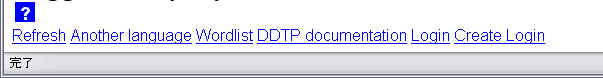
\includegraphics[scale=0.7]{image200906/ddtss129.jpg}

E メールアドレス (Email Address)とログイン名(Alias)、本名(Real Name)、パスワードを 2
回入力(Password, Retype Password)して Submit ボタンを押して送信すると、
アカウント作成は完了です。Alias は各種ログの表示で使われます、英文字のわ
かりやすい表記にしましょう。

  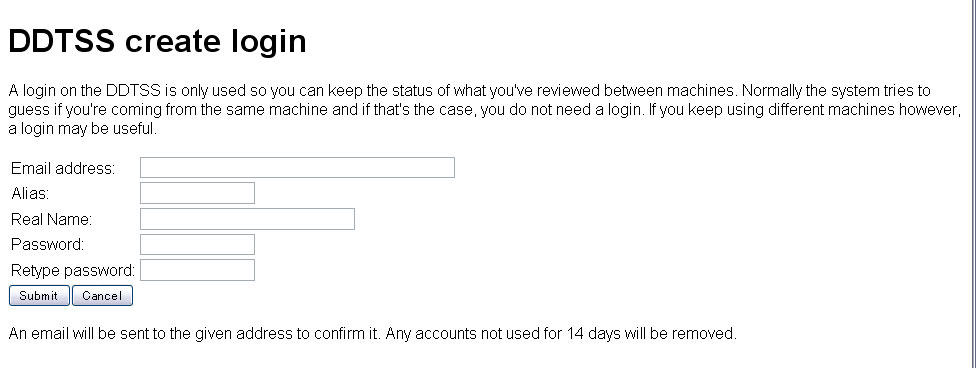
\includegraphics[scale=0.7]{image200906/ddtss141.jpg}

アカウントを作成したらログインします。作業画面の右上にアカウントの情報が表示されます。

  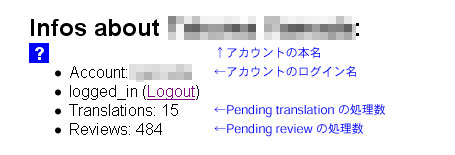
\includegraphics[scale=0.7]{image200906/ddtss130.jpg}

\subsection{DDTSS で行ってほしい作業 - レビュー}

現在 DDTSS でもっとも必要な作業は「レビュー」です。レビューの対象は、次の場所に表示されています。

\begin{commandline}
Pending review (98)

   1. bristol (needs initial review)
   2. pngquant (needs initial review)
   3. adesklets (needs initial review)
   4. inventor-demo (needs initial review)
   5. emboss (needs review, had 1)
\end{commandline}

パッケージ名をクリックすると内容が表示されます。その内容を見て、簡単そうならレビューをします。
難しいと思ったら、次のパッケージへ飛ばしてかまいません。

  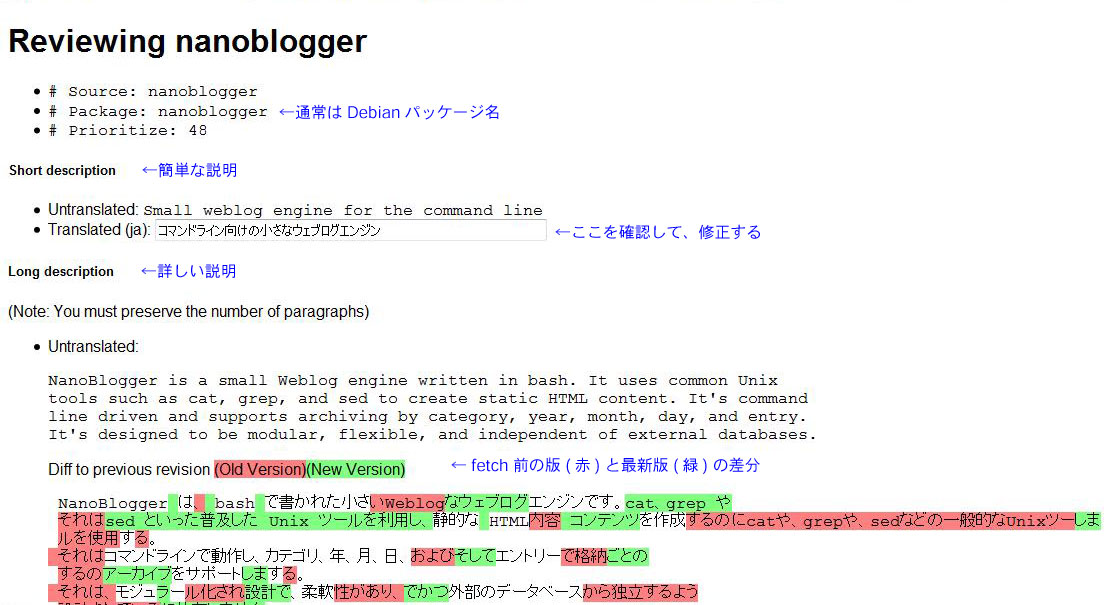
\includegraphics[width=170mm]{image200906/nanoblogger101.jpg}

  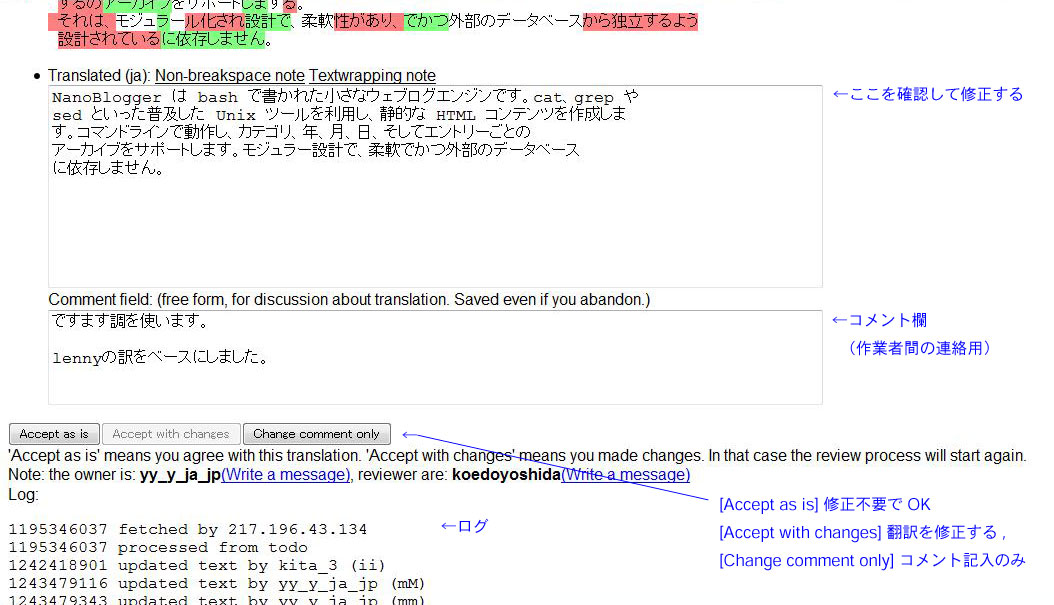
\includegraphics[width=170mm]{image200906/nanoblogger102.jpg}

  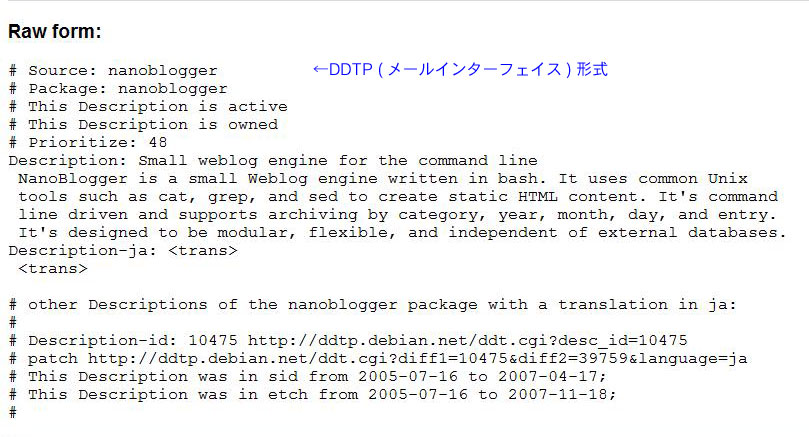
\includegraphics[width=130mm]{image200906/nanoblogger104.jpg}

\subsection{レビューする}

翻訳内容に問題ないと判断できた場合は、[Accept as is] ボタンをクリックしてください。

  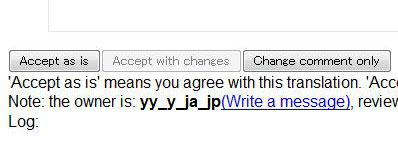
\includegraphics[scale=0.7]{image200906/nanoblogger112.jpg}

レビューをすると、表示される場所が変わります。さらにレビューが必要な場合
は、次のようになります。

  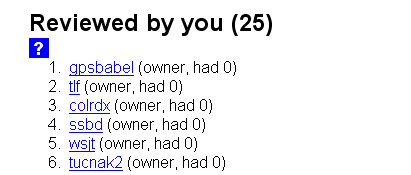
\includegraphics[scale=0.7]{image200906/ddtss131.jpg}

連続して 3 人がレビューをすると、翻訳作業が完了します.完了後は次のように
なります。

  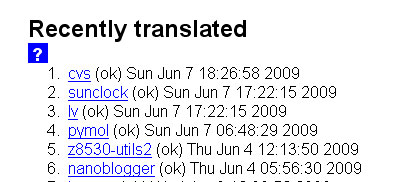
\includegraphics[scale=0.7]{image200906/ddtss132.jpg}

途中で誰かが翻訳を修正したら、再び 3 人のレビューが必要になります。

\subsection{レビューを修正する}

翻訳内容にすぐ修正が必要なら、テキストを変更してから [Accept with
changes] ボタンをクリックしてください。なるべくコメント欄 (Comment
field) に変更内容を記入してください。

  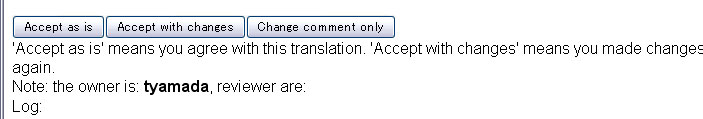
\includegraphics[scale=0.7]{image200906/ddtss145.jpg}

\subsection{翻訳を新規に作成する}

翻訳を新規に作成する場合は Pending Translation から選択してください。
レビューの際と違うのは、選択肢が Abandon (翻訳を中止する)と Submit (翻訳
を確定しレビューにまわす)の二つになっている点です。

\subsection{debian-doc ML へのお誘い}

翻訳の内容に疑問があったり、相談が必要だと思ったり、レビューや修正で 
(小さくない) 変更があったら、debian-doc ML に流してください。

debian-doc ML の宛先は、\url{debian-doc@debian.or.jp}

参加方法は、\url{http://www.debian.or.jp/community/ml/openml.html#docML}


質問や相談はフリーフォーマットです。

レビューを依頼するときは、次のメール例を参考にしてください。

(メールの例)

\begin{commandline}
Subject: DDTSS レビュー icedax

xxxです。

xxxx さんが修正した icedax をレビューしました。


Short description

原文: Creates WAV files from audio CDs
訳文: オーディオ CD から WAV を生成する

Long description

原文:
icedax lets you digitally copy ("rip") audio tracks from a CD, avoiding
(略)

訳文:
icedax により、CD からディジタルでオーディオトラックのコピー ("リッピング")
(略)

用語を一部修正しました。
ディジタル->デジタル

修正後:
icedax により、CD からディジタルでオーディオトラックのコピー ("リッピング")
(略)

修正処理をしましたので、内容の確認をお願いします。
\end{commandline}


\subsection{debian-doc ML だけでレビューする}

「DDTSS をやる時間がないよ」という方は、
debian-doc ML に流れているレビューや翻訳完了のメールを確認して、
何か問題が見つけたらメールに返信してください。
きっと誰かが DDTSS に反映するでしょう。

\subsection{最後に}

DDTSSは仕組み上レビューが大量に必要になります。
多くの人が参加していることが前提になっています。
なので、翻訳が正しい内容なのかを利用者の視点でレビューしてくれると助かります。

% ===============================================================
\dancersection{Debian GNU/kFreeBSD をインストールしてみよう}{山本 浩之}
\index{kfreebsd}
\index{debian}
% ===============================================================

今年 4 月 5 日に正式に Debian archive に入った Debian GNU/kFreeBSD ですが、
現時点で最新インストーラである debian-20090117-kfreebsd-i386-install.iso 
(2009/1/17製) を使ってインストールしてみました。

英文ドキュメント
http://glibc-bsd.alioth.debian.org/doc/

\begin{commandline}
wget http://glibc-bsd.alioth.debian.org/install-cd/kfreebsd-i386/current/debian-20090117-kfreebsd-i386-install.iso
\end{commandline}

このイメージにある kernel は、FreeBSD 7.1R のものですが、インストール後、
7.2R の kernel にアップグレード可能です。

今回は VMware の仮想ディスクにインストールを試みました。
インストーラは、現在のところは、FreeBSD 用のものを一部改造したもの
のようです。
インストーラを CD イメージから起動します。とりあえず Express (または Custom)で
インストールしてみましょう。
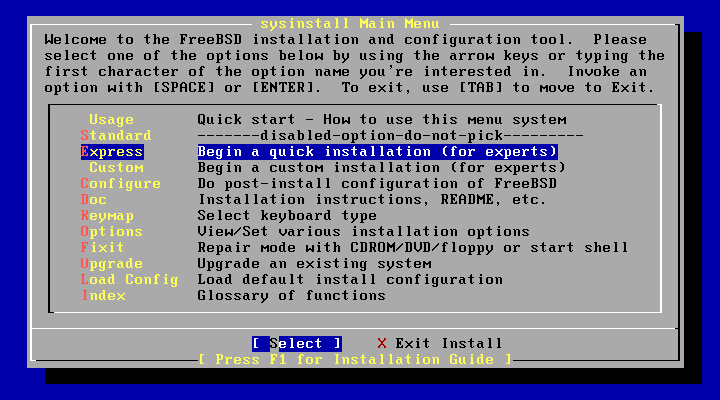
\includegraphics[width=6cm]{image200906/kfreebsd02.png}

まず最初にすることは、Linux と同様、インストールするディスクを指定します。
fdisk が起動しますが、ここで注意しなくてはならないのは、Linux とはディスクの
指定の仕方が違うことです。FreeBSD では、hda1 にあたるものは、ad0s1 で、
スライスと呼びます。FreeBSD では伝統的に、使用する領域全部を先にスライス (ad0s1) として確保し、
その中にディスクラベルをつけることによって小分けして(ad0s1a、ad0s1b など)、
それぞれのマウントポイントを作ります。
Linux の場合のパーティションの設定に近いものはディスクラベルかもしれません。
とりあえず "A" で、空き領域全部指定しましょう。
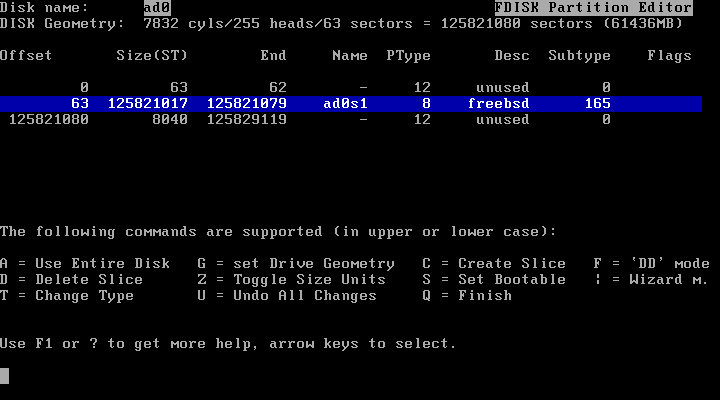
\includegraphics[width=6cm]{image200906/kfreebsd03.png}

次にブートローダの書き込みですが、デフォルトでは FreeBSD Boot Manager と言う
 FreeBSD 専用のプログラムが使用されます。もし既存の grub が使いたい場合には、
ここでは書き込まず (None を指定)、インストール後に、既存の grub が使っている 
/boot/grub/menu.lst に
\begin{commandline}
title Debian GNU/kFreeBSD
root (hd0,0,a)
kernel /boot/loader
\end{commandline}
とか書けば良いそうです。
仮想ディスクなどに対してのインストールで、マルチブートの必要が無い時は "Standard" を選んでください。
FreeBSD Boot Manager を使ってマルチブートしたい場合にのみ "BootMgr" を選んでください。
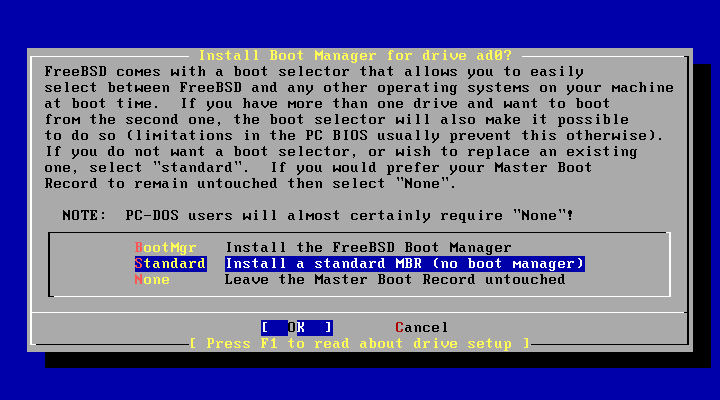
\includegraphics[width=6cm]{image200906/kfreebsd04.png}

次に FreeBSD Disklabel Editer が起動し、スライスの中に、
さらにマウントポイントとしていくつもディスクラベルをつけます。
それぞれ ad0s1a ad0s1b ...などとなります。
"/" のため、少なくとも一つはディスクラベルをつける必要があります。
もし、"/usr" とか "swap" とかを分けたいときにはここで選びます。
"A" で、自動的に割り振ることも可能です。
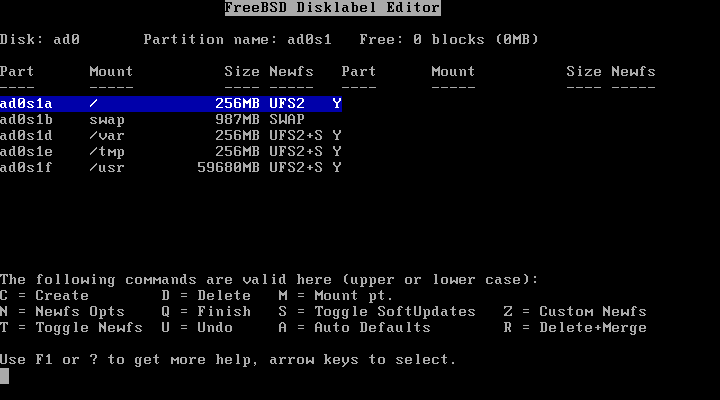
\includegraphics[width=6cm]{image200906/kfreebsd05.png}

そして Distribution の選択 (Choose Distribution) ですが、
ここでは必ず "A Minimal" を選択してください。
ここで色々な選択肢が出てきますが、これは元の FreeBSD のインストーラだったころの名残りで、
これは Debian のインストーラですから、FreeBSD の Distribution は全く収録されていません。
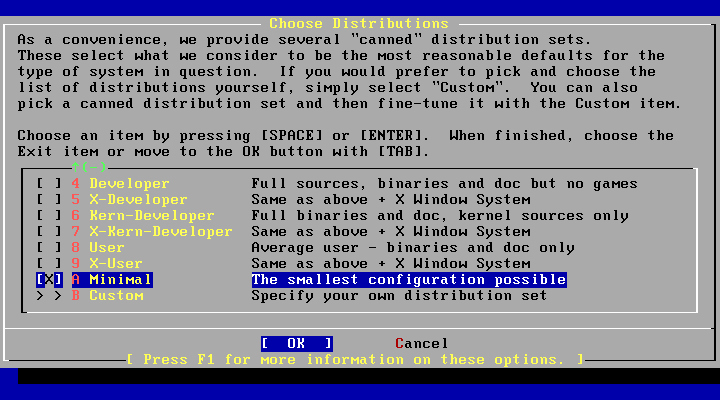
\includegraphics[width=6cm]{image200906/kfreebsd06.png}

次はイントールメディアの選択 (Choose Installation Media) ですが、
ここでは必ず "1 CD/DVD" を選択してください。
その他の選択肢は FreeBSD のインストーラだったころの名残りです。
自分の環境にあわせ、"cd0" (SCSI) または "acd0" (ATAPI) を選べば、
インストールの始まりです。
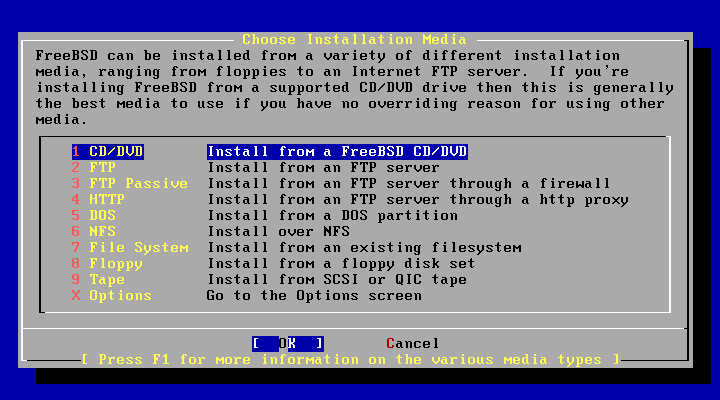
\includegraphics[width=6cm]{image200906/kfreebsd07.png}
途中で、"Alt-F3" を押すよう指示がありますから、それに従うと、
Debian GNU/Linux でお馴染みな、タイムゾーンの設定とか popularity-contest 
の設定とかができます。
Debian GNU/kFreeBSD 特有なものは、module-init-tools の設定で、
これは FreeBSD カーネルのモジュール名を選ばなければなりません。
ネットワークカードモジュールとサウンドカードモジュールとその他のモジュールが出てきますが、
詳しくは FreeBSD 本家のドキュメントを見てください。
私の場合は VMware ですので、サウンドカードモジュールの "snd\_es137x" のみ選びました。
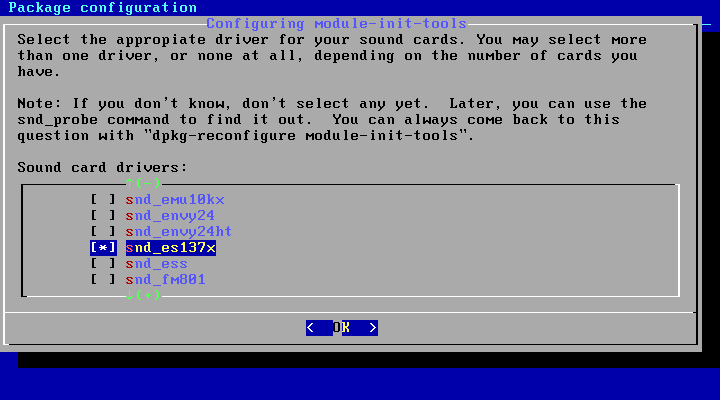
\includegraphics[width=6cm]{image200906/kfreebsd12.png}

最初の画面に戻ってきたらインストールは終わりです。
タブキーで "X Exit Install" を選び、再起動して下さい。

最初は root ユーザのみがパスワード無しで出来ています。
ユーザ名 root を入力すると、パスワードをきかれずにログインできます。

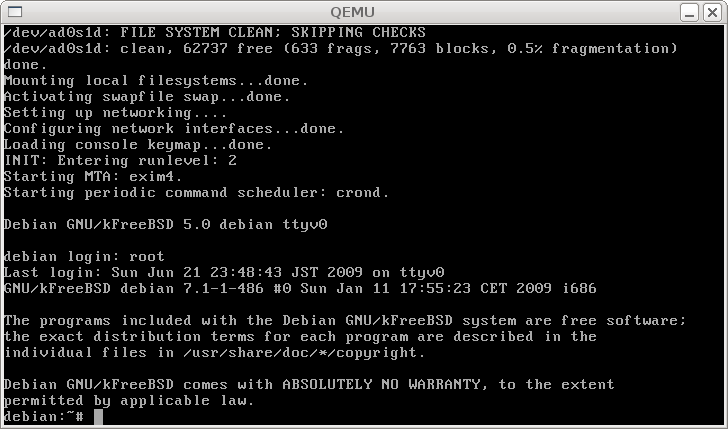
\includegraphics[width=6cm]{image200906/kfreebsdlogin.png}

root でログインしたら、まずはpasswdコマンドでパスワードを変更しましょう。
\begin{commandline}
passwd
\end{commandline}

次にネットワークの接続をします。
Linux の eth0 にあたるものは le0 (VMware の場合) または ed0 (Qemu の場合) 
のようです。
dhcp3-client パッケージは既にインストール済みのはずですから、DHCP 環境
\footnote{qemu の場合デフォルトでは dhcp でIPアドレスが取得できます}の人は /etc/network/interfaces を編集しなくても
\begin{commandline}
dhclient3
\end{commandline}
でネットワークに繋がるはずです。

固定 IP の人は、以下を参考にして、それぞれのファイルを編集して下さい。
\begin{commandline}
##/etc/network/interfaces の例
auto lo0
iface lo0 inet loopback
## Static network
auto le0
iface le0 inet static
    address 192.168.0.3
    network 192.168.0.0
    netmask 255.255.255.0
    gateway 192.168.0.1
\end{commandline}
\begin{commandline}
##/etc/resolv.conf の例
nameserver 192.168.0.1
\end{commandline}
その後、
\begin{commandline}
ifup le0
\end{commandline}
で、ネットワークに繋いで下さい。

インターネットに繋がったら、まず keymap の設定のため、
\begin{commandline}
apt-get update
apt-get install kbdcontrol
\end{commandline}
をして、console の keymap を選んでください。(console-data は使えません)

インストール後は、Debian GNU/Linux とどこが違うのか分からない程、まさに Debian です。

\subsection{参考文献}

\begin{itemize}
 \item Installing Debian GNU/kFreeBSD
       \url{http://glibc-bsd.alioth.debian.org/doc/}: インストール方法が
       詳しく記載されています。
\end{itemize}

\clearpage

%\printindex

\cleartooddpage

\vspace*{15cm}
\hrule
\vspace{2mm}

\includegraphics[width=2cm]{image200502/openlogo-nd.eps}
\noindent \Large \bf Debian 勉強会資料\\ \\
\noindent \normalfont \debmtgyear{}年\debmtgmonth{}月\debmtgdate{}日 \hspace{5mm}  初版第1刷発行\\
\noindent \normalfont 東京エリア Debian 勉強会 (編集・印刷・発行)\\
\hrule


\end{document}
